The two sequential methods are implemented as separate functions that are called from within a while loop in the main file. The while loop runs as long as the checksum is larger than the threshold, $d$, AND while the number of iterations, $k$ is smaller than a user-specified $k_\mathrm{max}$:
\begin{lstlisting}
while(checksum > d && k < kmax)
\end{lstlisting}
The checksum is defined as the Frobenius norm of the difference between the updated matrix and the previous version of the matrix. The norm is
\begin{equation}
||u-u_O||_F = \equiv \sqrt{\sum_i\sum_j (u_{i,j}-u_{O, i,j})^2}.
\end{equation}
The functions are implemented in a straight-forward way with a double for loop. The input variables are the new matrix, $u$, the old matrix, $uo$, the source matrix, $f$, the size of the matrices, $N$, and the grid spacing squared $\Delta ^2$. The loops run from $1$ to $N-2$ such that the edge of the matrices are not updated.
\begin{lstlisting}[caption = Implementation of the sequential Jacobi iterative process]
void jacobi_seq(double ** u, double ** uo, double ** f, int N, double delta2){

	int i,j;
	for(i = 1; i < N-1; i++){
		for(j = 1; j < N-1; j++){
			u[i][j] = 0.25*(uo[i-1][j] + uo[i+1][j] + uo[i][j+1] + uo[i][j-1] + delta2*f[i][j]);
		}
	}
}
\end{lstlisting}

\begin{lstlisting}[caption = Implementation of the sequential Gauss-Seidel iterative process]
void gauss_seidel(double ** u, double ** f, int N, double delta2){

	int i,j;
	for(i = 1; i < N-1; i++){
		for(j = 1; j < N-1; j++){
			u[i][j] = 0.25*(u[i-1][j] + u[i+1][j] + u[i][j-1] + u[i][j+1] + delta2*f[i][j]);
		}
	}
}
\end{lstlisting}

\subsection{Comparing convergence}
The two functions are run with a fixed size of $N=100$, and $k_\mathrm{max}$ large enough that the clause that stops the while loop is always the convergence criterion. The threshold is varied from $10^{-1}$ to $10^{-11}$, and the resulting number of iterations until convergence fro the two functions is seen in figure \ref{fig:itd}. The $x$-axis is logarithmic, so the behavior is exponential, and the Gauss-Seidel is approximately twice as fast as the Jacobi method. The black dashed line is Jacobi line divided by two, and it follows the Gauss-Seidel line with a slight off-set, but the slopes are identical.

\begin{figure}
\centering
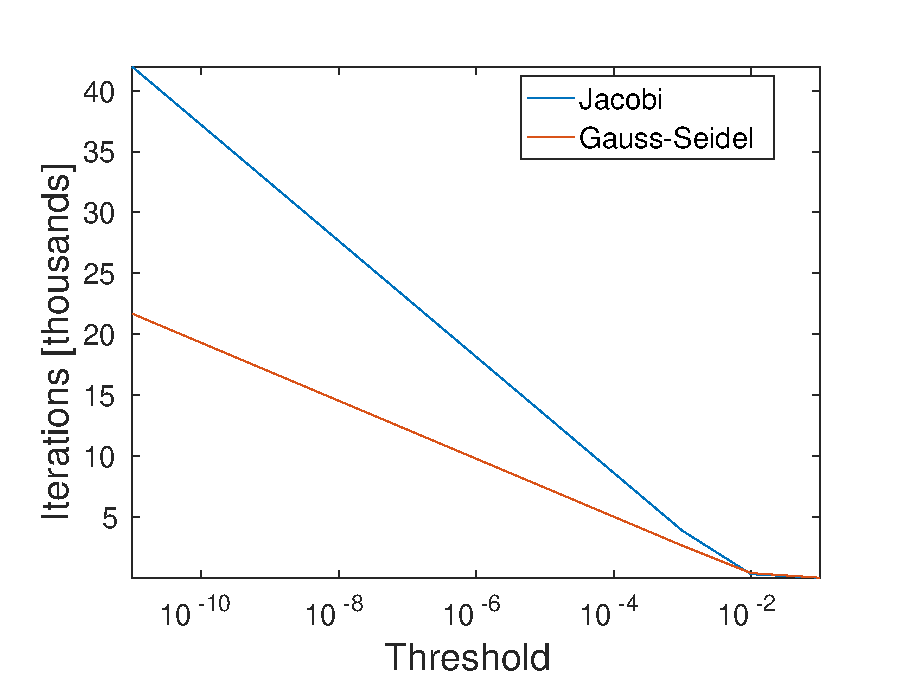
\includegraphics[width = 0.8\textwidth]{fig/itd_jac_gs.eps}
\caption{The convergence of the Jacobi method and the Gauss-Seidel method with changing threshold.}
\label{fig:itd}
\end{figure}

The convergence is now investigated as a function of matrix size, $N$. For a constant threshold, the matrix size is varied, and the number of iterations required to converge is reported. The result can be seen in figure \ref{fig:itN}. We expected the initial increase to continue steadily for all matrix sizes, but as seen, the curves have a maximum depending on the threshold $d$. This can be explained by the fact that the Frobenius norm is the average norm of all points in the matrix. The first order central difference scheme only uses the next neighbors, and so, the change of $u$ happens like a wave coming from the edges with the boundary conditions and the points where $f \neq 0$. This means that only the points where the wave is has notable differences between $u$ and $u_O$. For example, the points in the center of the domain is initialized to zero, and they will remain that for approximately $N/2$ iterations before the change gets to the center. This implies that the norm of the center of the domain is zero, significantly lowering the total norm. After many iterations, the points near the sides of the domain have all converged, and the norm of these points will lower the total norm as well. This means that when the matrix size is increased, so is the number of points in the center which does not change in the beginning, and the norm is lowered to a point where the program thinks the problem has converged, but in reality it has not. For smaller thresholds, the size where the decrease in iterations happen will increase, but the general behavior is identical. This implies that when using the Frobenius norm, one must make sure that the threshold and the size are such that it is on the increasing part of figure \ref{fig:itN} in order to be sure that the result is indeed the correct result. Alternatively, one could initialize the $u$ and $u_O$ arrays to random numbers, but that would require a lot of extra computations to be done. Another solution is to compare the change in each element with the threshold, but that requires an if-clause for each element, which also reduced performance significantly. Finally, it should be noted that the performance of the subsequent sections are still valid because it only compares timings and scaling behavior and not the result of the computation.

\begin{figure}
\centering
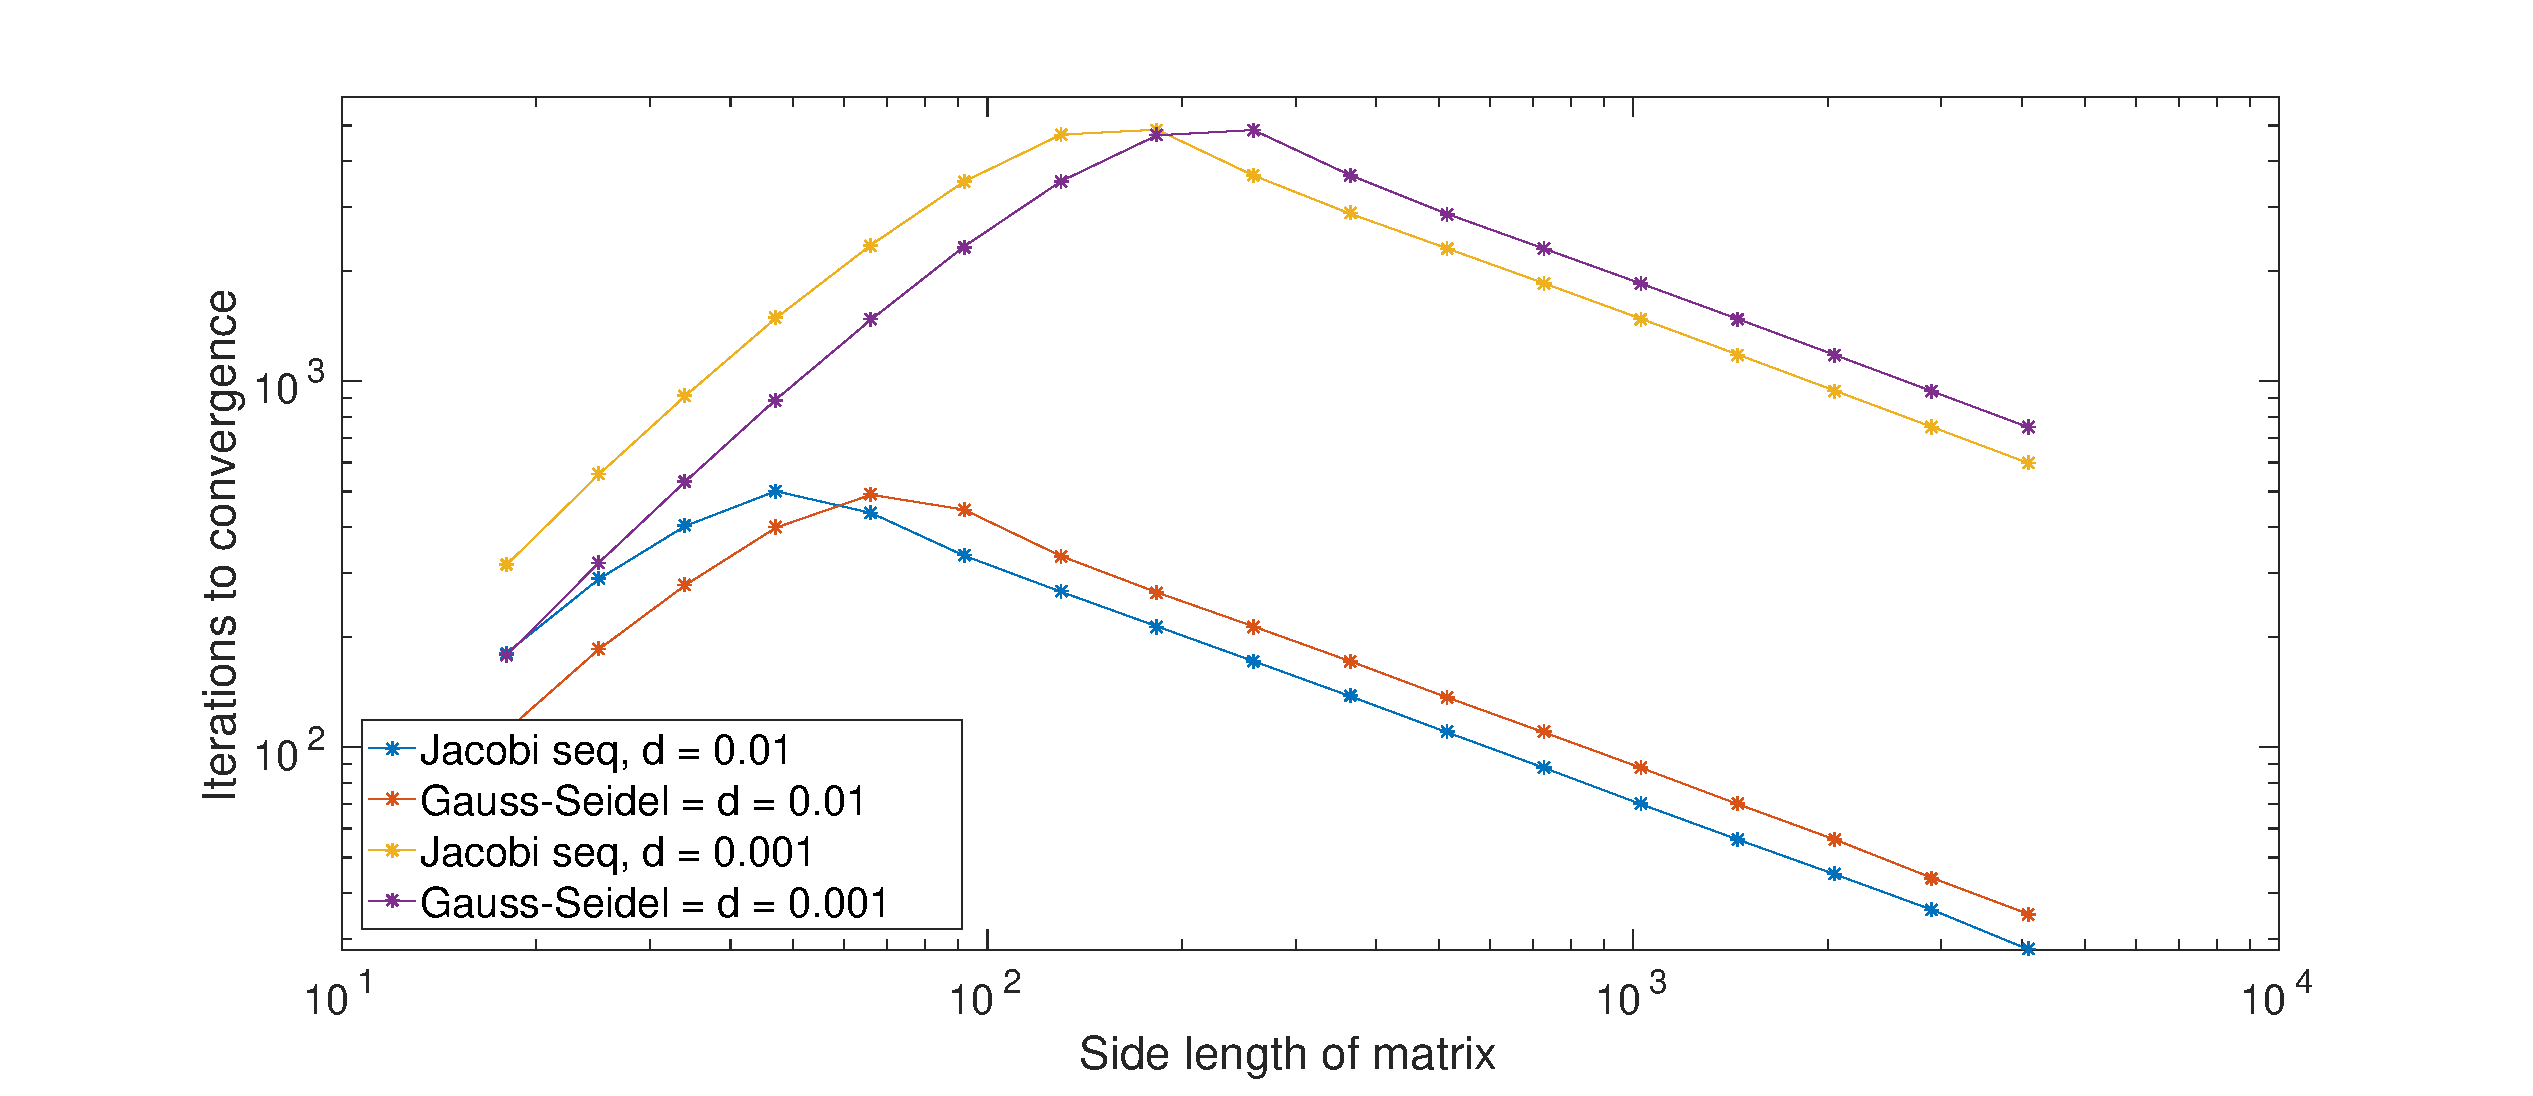
\includegraphics[width = 1.1\textwidth]{fig/itN.eps}
\caption{The convergence of the Jacobi method and the Gauss-Seidel method with changing matrix size.}
\label{fig:itN}
\end{figure}

\subsection{Comparing performance}
The performance of the two sequential functions are analyzed by comparing the number of point updates per second. The program is forced to run for at least three seconds to get a reliable timing. The resulting graphs is shown in figure \ref{fig:seq_perf}. For small matrices the Jacobi method is $\sim$ twice as fast as the Gauss-Seidel method. This is due to the fact that the Gauss-Seidel method read and write in the same array, which cause some memory "clogging" in the caches. For matrices exceeding the L3 cache, the Jacobi method slows down significantly, due to the smaller bandwidth to/from memory compared to the caches. The Gauss-Seidel method is reduced as well for the same reasons, but not nearly as significantly due to the memory clogging already taking place in the caches. However, as seen on figure \ref{fig:itd}, the Gauss-Seidel method requires half as many iterations to converge to the same precision, making it faster in wall clock time.

\begin{figure}
\centering
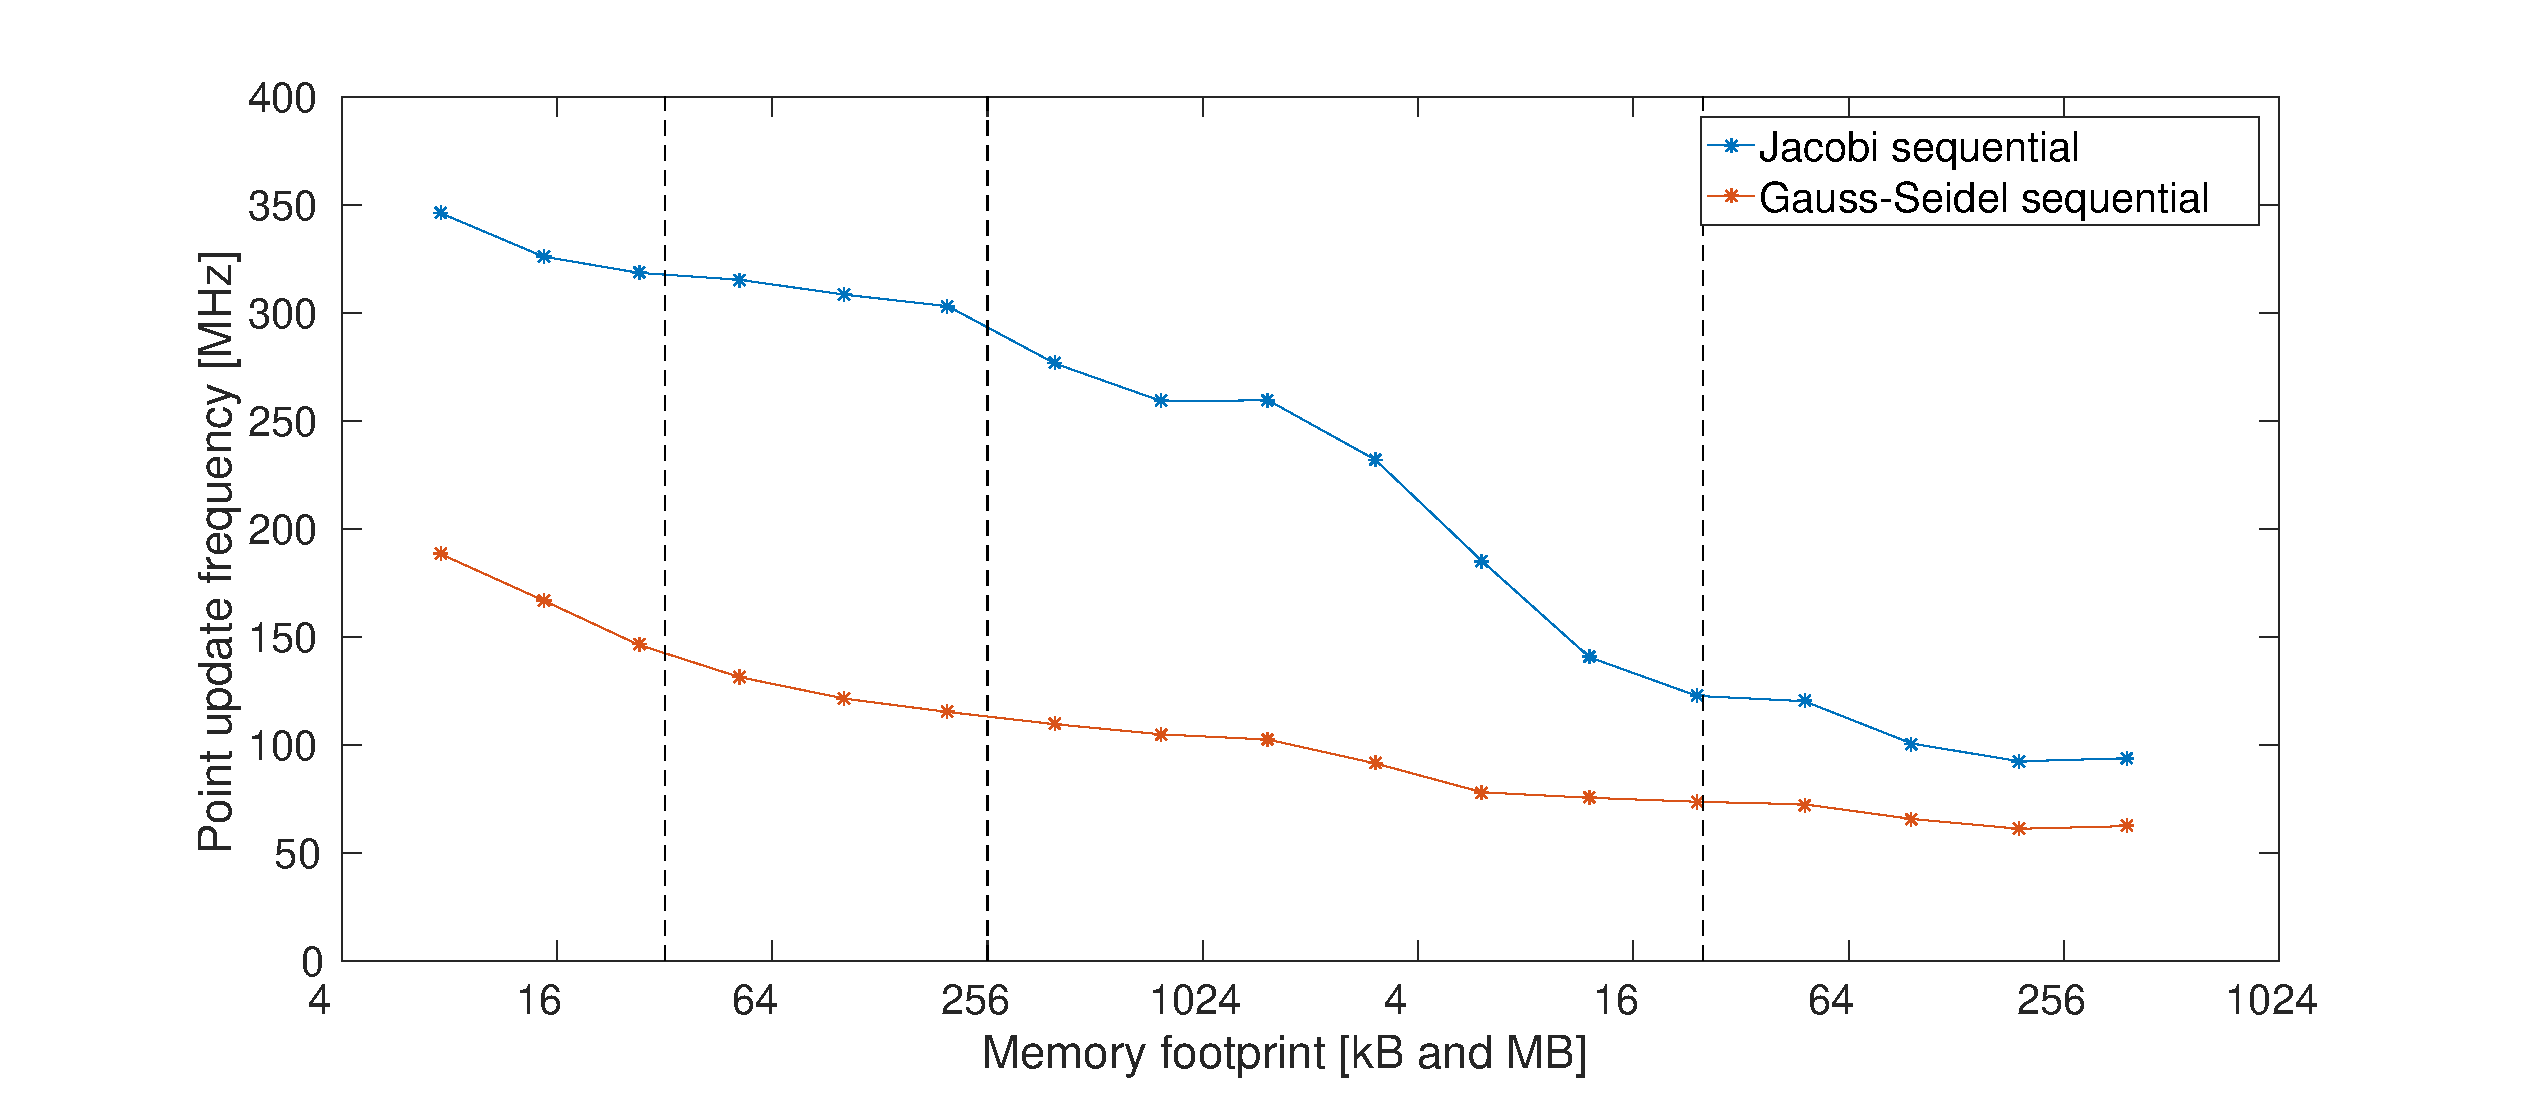
\includegraphics[width = 1.1\textwidth]{fig/seq_perf.eps}
\caption{The performance of the two sequential functions with changing domain size. The black dashed lines represent the cache sizes of the CPU.}
\label{fig:seq_perf}
\end{figure}